\documentclass[12pt]{article}
\usepackage{graphicx,psfrag,amsfonts,float,mathbbol,xcolor,cleveref}
\usepackage{arydshln}
\usepackage{amsmath}
\usepackage{tikz}
\usepackage[mathscr]{euscript}
\usepackage{enumitem}
\usepackage{accents}
\usepackage{framed}
\usepackage{subcaption}
\usepackage{natbib}
\usepackage{mathtools}
\usepackage{IEEEtrantools}
\usepackage{times}
\usepackage{cite}
\usepackage{amsthm}
\usepackage[letterpaper, left=1in, top=1in, right=1in, bottom=1in,nohead,includefoot, verbose, ignoremp]{geometry}
\usepackage{booktabs}
\newcommand{\ra}[1]{\renewcommand{\arraystretch}{#1}}
\newcommand{\comment}[1]{\text{\phantom{(#1)}} \tag{#1}}
\newcommand\numberthis{\addtocounter{equation}{1}\tag{\theequation}}
\newcommand*\needsparaphrased{\color{red}}
\newcommand*\needscited{\color{orange}}
\newcommand*\needsproof{\color{blue}}
\newcommand*\outlineskeleton{\color{green}}
\newcommand{\PP}{\mathcal{P}}
\newcommand{\bfeps}{\mbox{\boldmath $\epsilon$}}
\newcommand{\bfgamma}{\mbox{\boldmath $\gamma$}}
\newcommand{\bflam}{\mbox{\boldmath $\lambda$}}
\newcommand{\bfphi}{\mbox{\boldmath $\phi$}}
\newcommand{\bfsigma}{\mbox{\boldmath $\sigma$}}
\newcommand{\bfbeta}{\mbox{\boldmath $\beta$}}
\newcommand{\bfalpha}{\mbox{\boldmath $\alpha$}}
\newcommand{\bfe}{\mbox{\boldmath $e$}}
\newcommand{\bff}{\mbox{\boldmath $f$}}
\newcommand{\bfone}{\mbox{\boldmath $1$}}
\newcommand{\bft}{\mbox{\boldmath $t$}}
\newcommand{\bfo}{\mbox{\boldmath $0$}}
\newcommand{\bfO}{\mbox{\boldmath $O$}}
\newcommand{\bfx}{\mbox{\boldmath $x$}}
\newcommand{\bfX}{\mbox{\boldmath $X$}}
\newcommand{\bfz}{\mbox{\boldmath $z$}}


\newcommand{\bfm}{\mbox{\boldmath $m}}
\newcommand{\bfy}{\mbox{\boldmath $y$}}
\newcommand{\bfa}{\mbox{\boldmath $a$}}
\newcommand{\bfb}{\mbox{\boldmath $b$}}
\newcommand{\bfY}{\mbox{\boldmath $Y$}}
\newcommand{\bfS}{\mbox{\boldmath $S$}}
\newcommand{\bfZ}{\mbox{\boldmath $Z$}}
\newcommand{\cardT}{\vert \mathcal{T} \vert}
%\newenvironment{theorem}[1][Theorem]{\begin{trivlist}
%\item[\hskip \labelsep {\bfseries #1}]}{\end{trivlist}}
%\newenvironment{corollary}[1][Corollary]{\begin{trivlist}
%\item[\hskip \labelsep {\bfseries #1}]}{\end{trivlist}}
%\newenvironment{proposition}[1][Proposition]{\begin{trivlist}
%\item[\hskip \labelsep {\bfseries #1}]}{\end{trivlist}}
%\newenvironment{definition}[1][Definition]{\begin{trivlist}
%\item[\hskip \labelsep {\bfseries #1}]}{\end{trivlist}}

\newtheorem{theorem}{Theorem}[section]
\newtheorem{lemma}[theorem]{Lemma}
\newtheorem{proposition}[theorem]{Proposition}
\newtheorem{corollary}[theorem]{Corollary}

\theoremstyle{definition}
\newtheorem{definition}{Definition}[section]
\newtheorem{example}{Example}[section]
\def\bL{\mathbf{L}}

\begingroup\lccode`~=`_
\lowercase{\endgroup\def~}#1{_{\scriptscriptstyle#1}}
\AtBeginDocument{\mathcode`_="8000 \catcode`_=12 }

\makeatletter
\renewcommand{\theenumi}{\Roman{enumi}}
\renewcommand{\labelenumi}{\theenumi.}
\renewcommand{\theenumii}{\Alph{enumii}}
\renewcommand{\labelenumii}{\theenumii.}
\renewcommand{\p@enumii}{\theenumi.}
\makeatother

\begin{document}

%\nocite{*}
\def\bL{\mathbf{L}}
%\usepackage{mathtime}

%%UNCOMMENT following line if you have package


\title{ Nonparametric Covariance Estimation for Longitudinal Data via Penalized Tensor Product Splines}

\author{Tayler A. Blake\thanks{The Ohio State University, 1958 Neil Avenue, Columbus, OH 43201} \and  Yoonkyung Lee\thanks{The Ohio State University, 1958 Neil Avenue, Columbus, OH 43201}}

\bibliographystyle{plainnat}
\maketitle

\section{Cattle weights}

Fitted models can be found in 
/Users/taylerblake/GitRepos/cautious-guacamole/cache/kenward-cattle-analysis.RData

See Kenward, Michael G. (1987). A Method for Comparing Profiles of Repeated Measurements. Applied Statistics, 36, 296-308. Table 1. http://doi.org/10.2307/2347788


\citet{kenward1987method} reported an experiment designed to investigate the impact of the control of intestinal parasites in cattle. During the grazing season which runs from spring to autumn, cattle can potentially ingest roundworm larvae, developed from eggs deposited around the pasture from feces of previously infected cattle. Immune resistance to disease is suppressed once an animal is infected and deprived of nutrients; consequently, animal growth can be greatly impacted. Monitoring the effect of a treatment for the disease requires repeated weight measurements on animals over the grazing season. 

To compare two methods for controlling the disease, say treatment A and treatment B, each of 60 cattle were assigned randomly to two groups, each of size 30. Animal subjects were put out to pasture at the start of grazing season, with each member of the groups receiving one of the two treatments. Animals were weighed $m = 11$ times over a 133-day period; the first 10 measurements on each animal were made at two-week intervals and the final measurement was made one week later. Weights were recorded to the nearest kilogram. The measurement times were common across animals and were rescaled to $t = 1, 2, \dots, 10, 10.5$. The longitudinal dataset is balanced, as there were no missing observations for any of the experimental units. Observed weights are shown in Figure~\ref{fig:cattle-weights-by-trt}.
  
\begin{figure}[h] \label{fig:cattle-weights-by-trt}
\caption{Subject-specific weight curves over time for treatment groups A and B.}
\centering
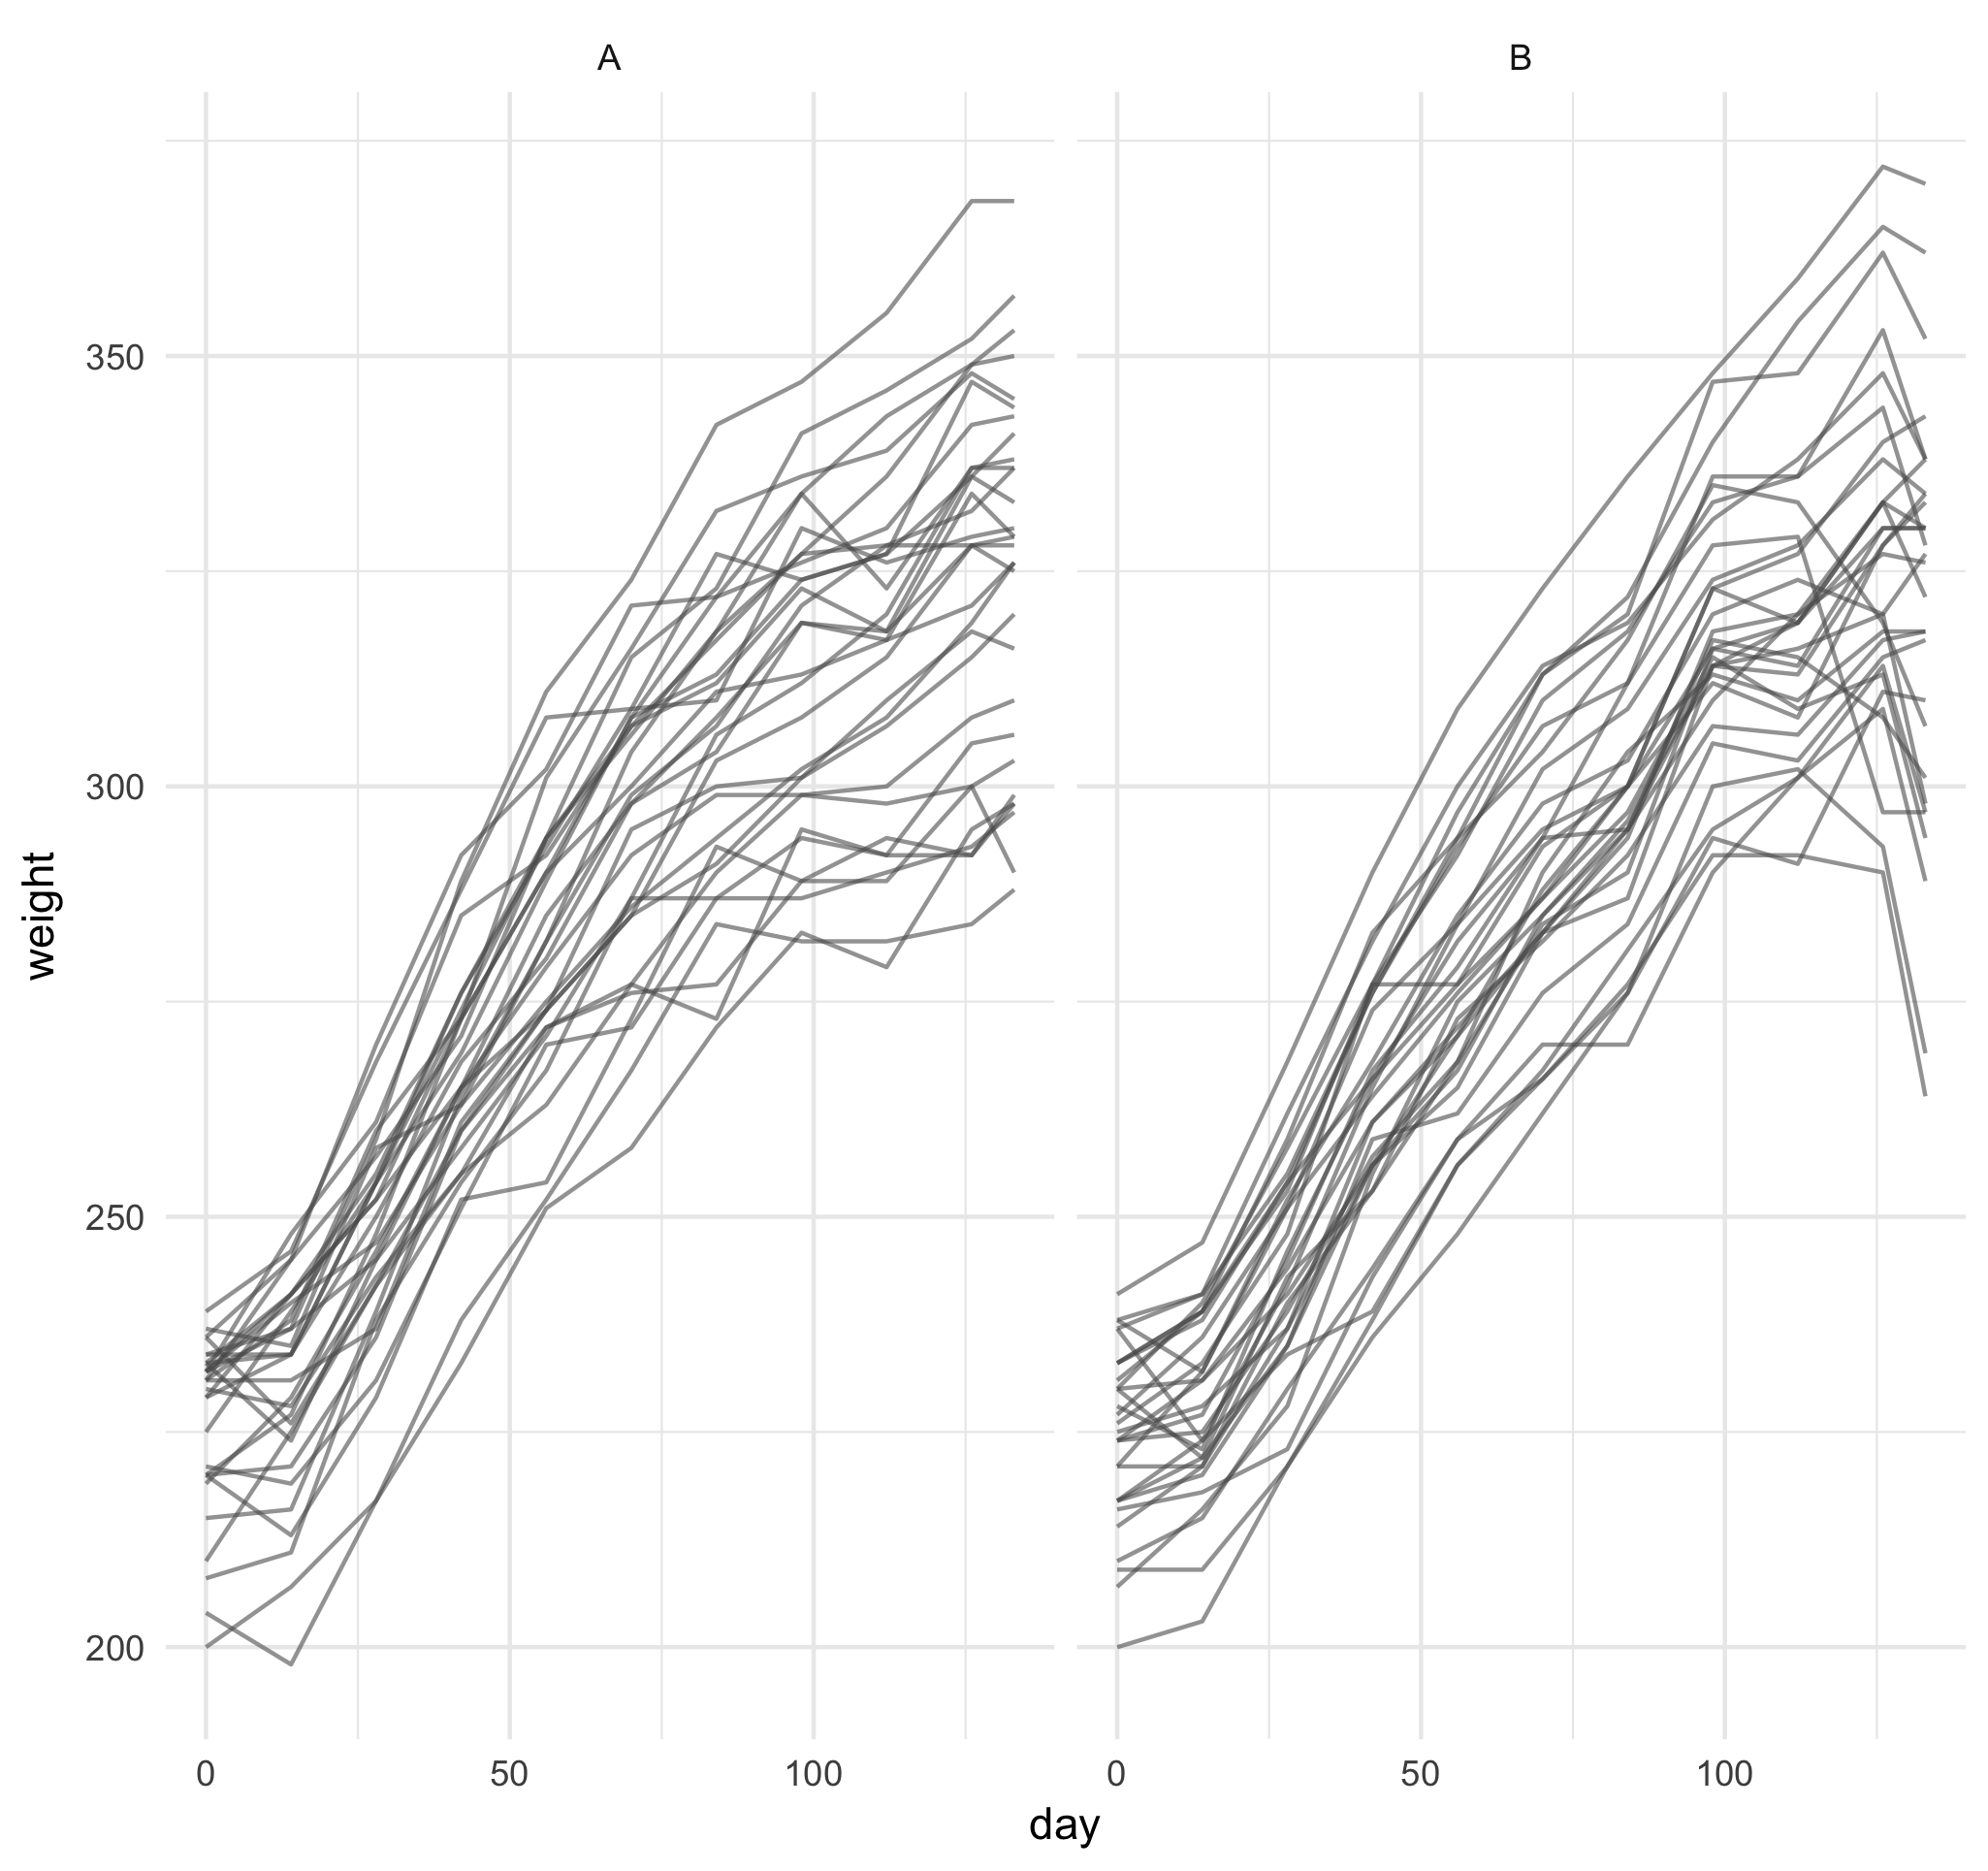
\includegraphics[width=0.5\textwidth]{cattle-weights-vs-time-by-trt.png}
\end{figure} 

\begin{figure}[h] \label{fig:cattleA-weights-fitted-mean-curve}
\caption{Fitted mean weight curve for cattle in treatment group A. The mean curve was modeled using a cubic smoothing spline; smoothing parameters were selected using the generalized maximum likelihood criterion.}
\centering
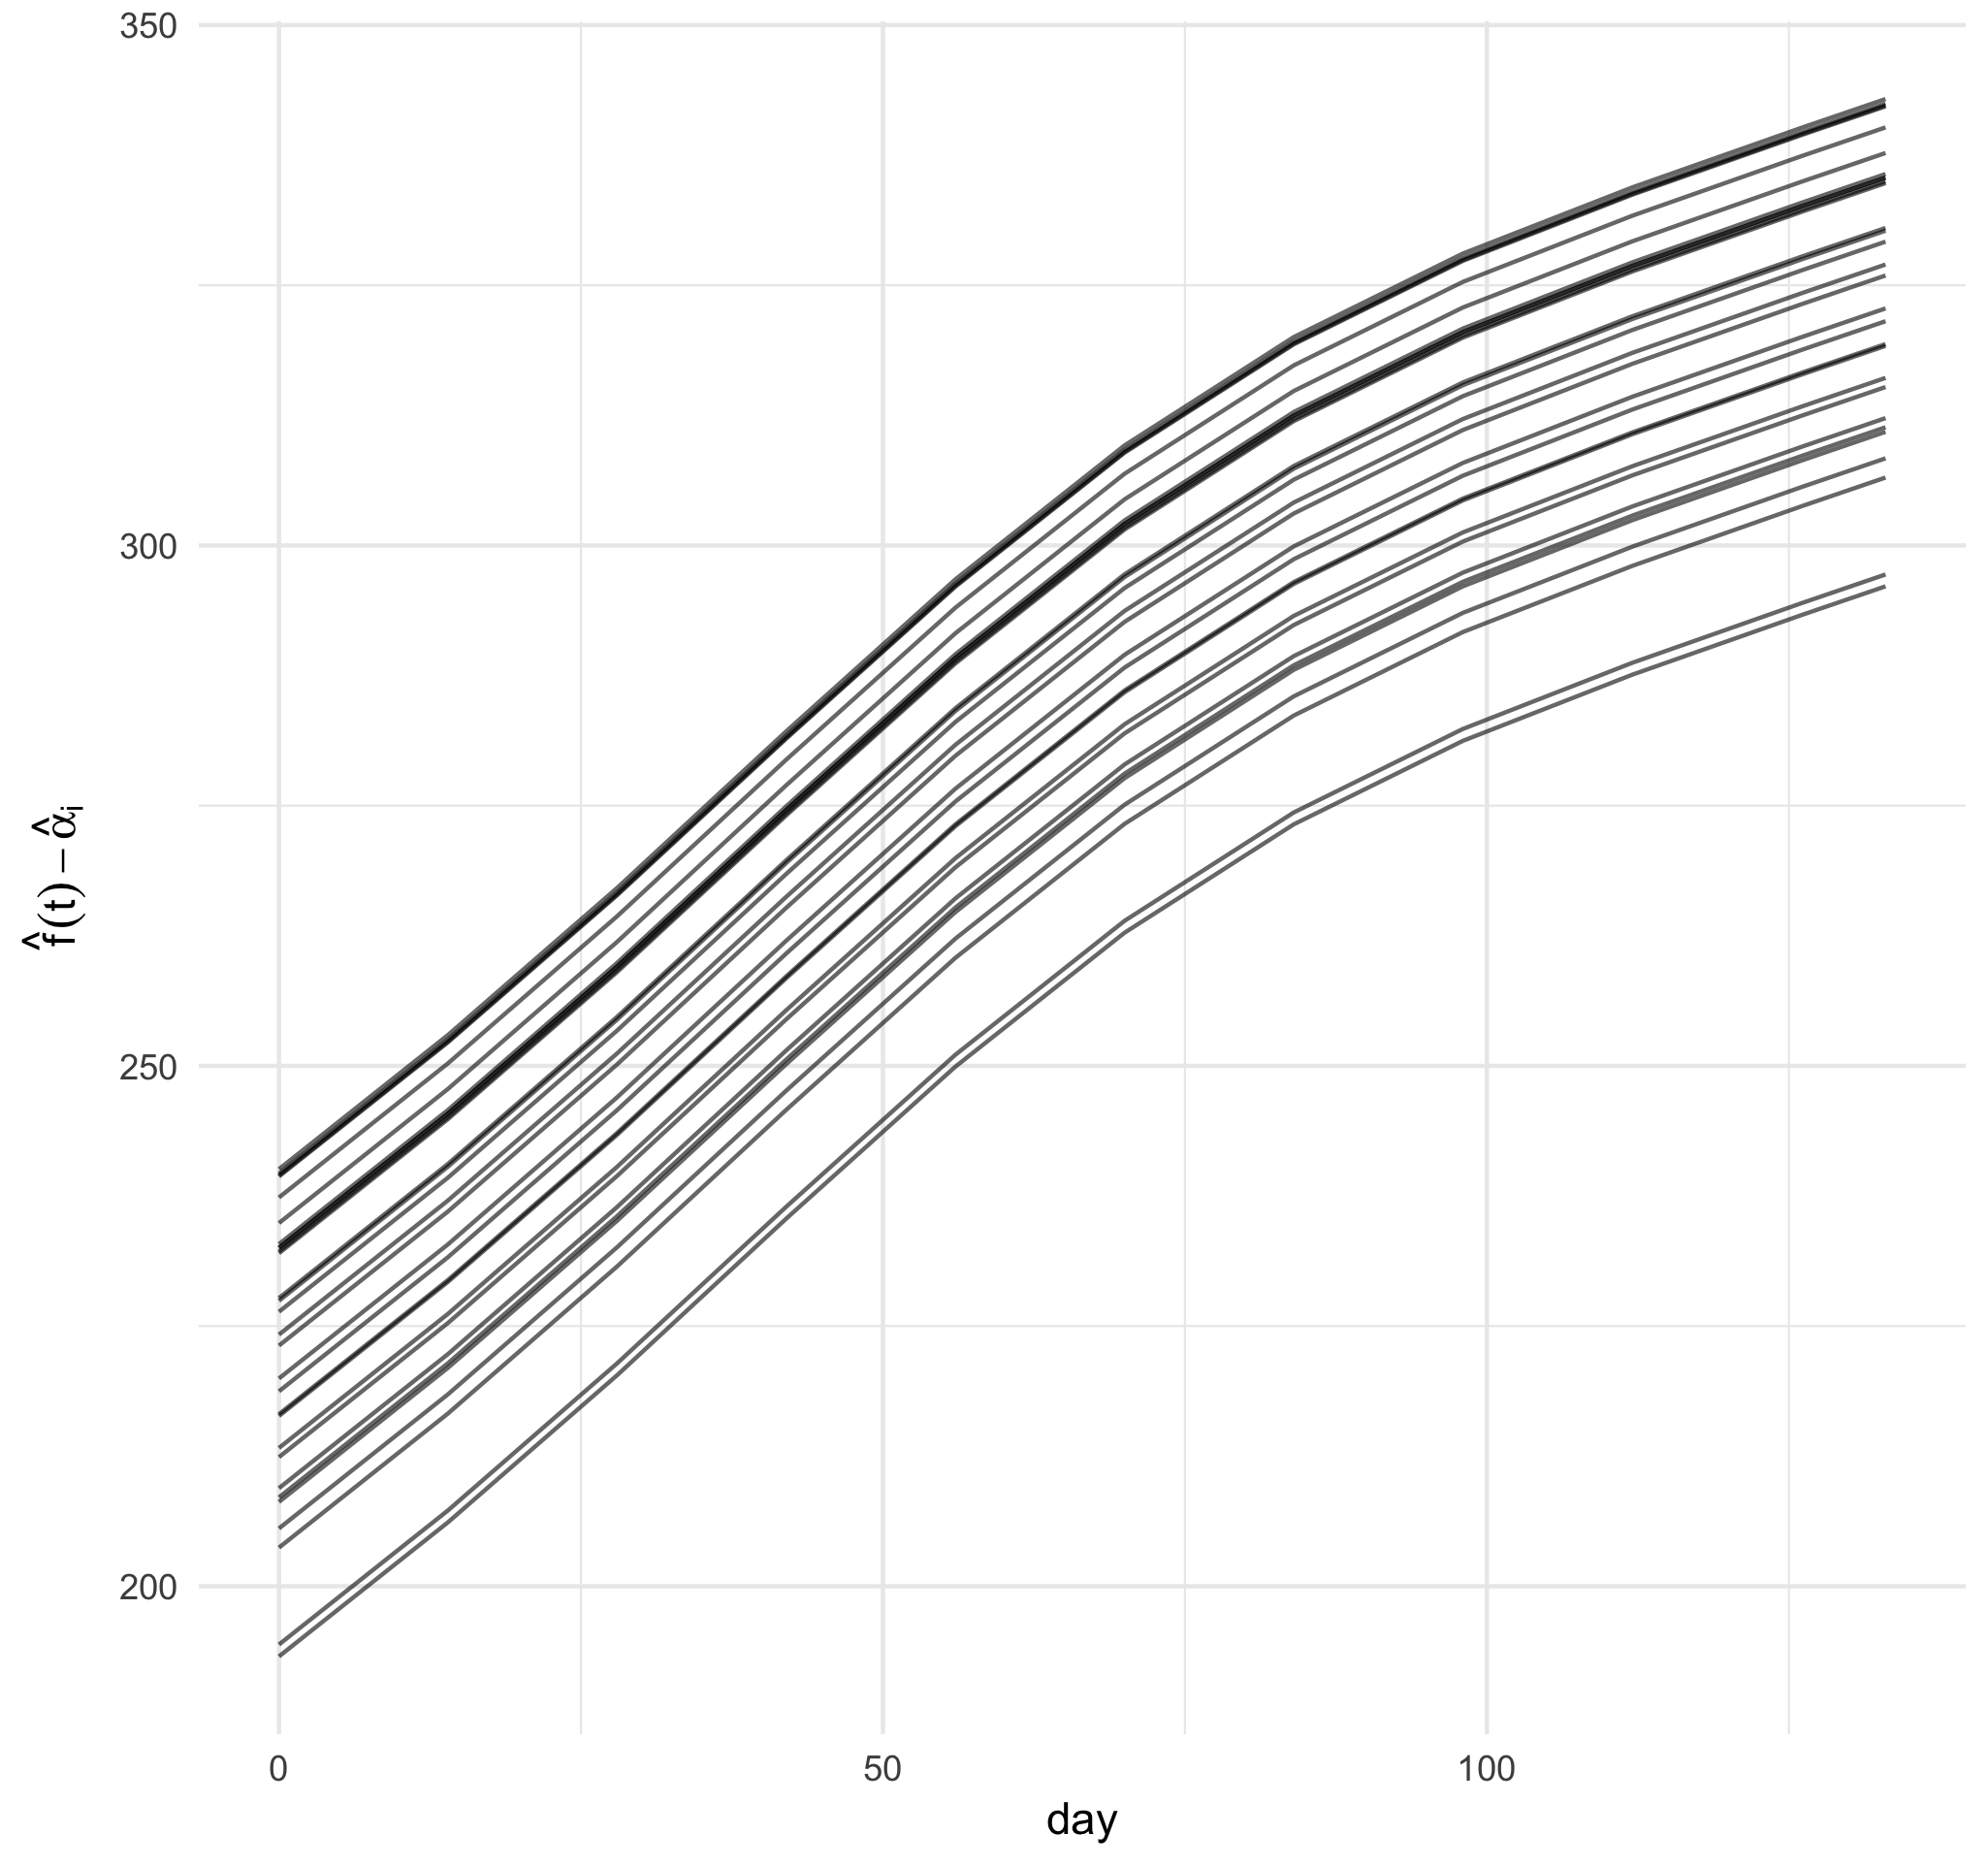
\includegraphics[width=0.5\textwidth]{cattleA-weights-vs-time-mean-fit.png}
\end{figure} 

We see an upward trend in weights over time, with variance in weights increasing over time for both groups. Treatment group B demonstrates a sharp decrease in the final weight measurement. The analysis provided by \citet{zimmerman1997structured} rejected equality of the two covariance matrices corresponding to treatment group using the classical likelihood ratio test, making it reasonable to study each treatment group?s covariance matrix separately. Following \citet{pan2017jmcm}, \citet{zhang2015joint}, \citet{pourahmadi1999joint}, and \citet{pan2006regression}, we analyze the data from cattle assigned to treatment group A. 

For the treatment group A with $N = 30$ animals, we assume a common mean function, $\mu\left(t\right)$ and an $11 \times 11$ covariance matrix $\Sigma$. A profile plot of the data reveals that the weights have an upward trend and their variances tend to increase over time, which suggests nonstationary covariance structure. This is confirmed by the upper diagonal entries in Table 1, which are the sample correlations. Furthermore, correlations within the subdiagonals are not constant and increase over time, giving a second indication that a stationary covariance is not appropriate for the data. Table 1 gives the sample correlations,  generalised autoregressive parameters and the innovation variances, and the latter two are plotted in Fig. 2(a), (c). These plots reveal that both the sample generalised autoregress
ive parameters and the logarithms of the innovation variances are cubic functions of the lag. That is, for t = 1, 2,..., 10, 11


\end{document}
